\doublespacing
\chapter{MARCO TEÓRICO}
\label{sec:marco teorico}
\spacing{1.5}
\lettrine[lines=4, slope=0.2em, findent=0.2em, nindent=0.6em]{E}l presente capitulo tiene como propósito presentar al lector algunas investigaciones y conceptos relacionados con IA, específicamente ML y en salud particularmente de ACV Isquémico, conceptos claves para esta investigación. \\
\par La organización del capítulo se encuentra de la siguiente manera, inicialmente, veremos ML y sus técnicas clásicas, pues consideramos estas podrían ser la respuesta a nuestra problemática junto a Deep Learning (DL), posteriormente nos enfocaremos en algunos términos de salud que nos ayudarán a entender de mejor forma el problema. 
\\

\doublespacing
\section{Inteligencia Artificial}
\spacing{1.5}
Las matemáticas nos han ayudado a interpretar y entender nuestro medio ambiente y ser capaz de predecir algunos sucesos en áreas como la cosmología o naturaleza o problemas incomprendidos por los humanos \cite{Grazia2022}. Hoy en día contamos con el área de las ciencias de la computación que fue creada hace solo un par de décadas atrás, siendo una de las ciencias más nuevas y que tiene gran valoración en la actualidad. En las ciencias de la computación podemos encontrar varias áreas aplicadas, de las cuales la IA destaca por su relación con la matemática, biología, lingüística, entre otras. \cite{Grazia2022}.\\
\par La IA llegó para resolver tareas que el ser humano realiza como tareas cotidianas básicas y complejas. Los algoritmos de IA se basan en el aprendizaje automático, siendo que cada vez las máquinas pueden aprender por ellas mismas algunas cosas, es así que los humanos dejaremos de perder nuestro tiempo programando reglas para lidiar con muchas combinaciones de datos y situaciones que se presentan a diario. Pues es así, que el aprendizaje de los propios algoritmos mejora el rendimiento de estos sin la necesidad de programación adicional por parte humana. Esto es logrado a través del uso de técnicas de aprendizaje automático, en las que el algoritmo es entrenado con un conjunto de datos y luego se ajusta a medida que recibe nuevos datos y realiza más tareas. \cite{Carola}.\\
\par En la IA, para que los modelos funcionen existen modelos neuronales y estos son los que determinan cómo se conectan los datos predictores con los objetivos a través de capas ocultas, y estas a su vez contienen unidades no observables \cite{IBM}. Dentro de la IA, convive un sub conjunto llamada ML y su vez, dentro de ML vive un subconjunto llamado DL. Estos sub conjuntos interactúan con lo que es el Data Science y el Big Data, haciendo de las aplicaciones una variada gama de aplicaciones \cite{moreno2021diseno}.\\

\begin{figure}[H]
	\centering
	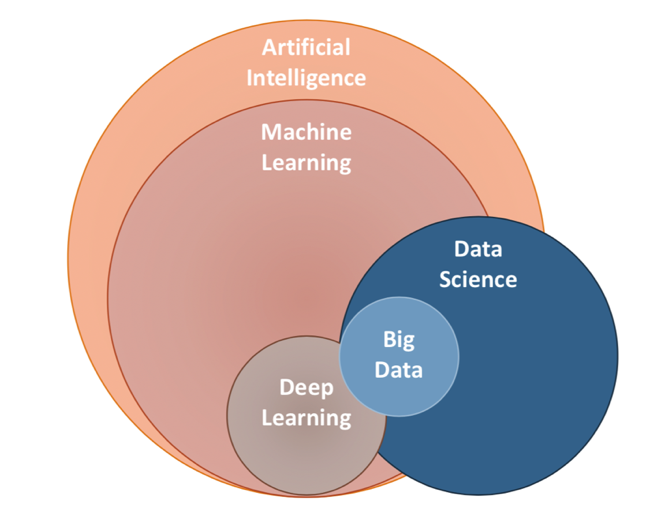
\includegraphics[scale=0.51]{img/Marco Teorico/Expertiz.png} 
	\caption{Diagrama de Venn con las subáreas de la IA}
\end{figure}


\doublespacing
\section{Machine Learning}
\spacing{1.5}
Los problemas por computadora se solucionan con un algoritmo que le indica a la máquina los pasos a seguir. En un ejemplo clásico podemos usar un algoritmo de búsqueda, donde el dato a buscar sería la entrada y su salida sería si se encontró o no y en cuánto tiempo. Es bien conocido que para resolver el problema de búsqueda existen variados algoritmos, algunos más eficientes que otros, aplicables a un contexto u otro de mejor forma, solucionando el mismo problema.\\
\par Asimismo, la publicidad en el celular es un ejemplo de cómo los algoritmos de ML están aplicándose en la vida cotidiana. Estos algoritmos utilizan técnicas de análisis de datos y aprendizaje automático para comprender los patrones de comportamiento y preferencias de los usuarios a partir de la información de navegación y otros datos recopilados en sus dispositivos móviles. Además de la publicidad en el celular, los algoritmos de ML también están siendo utilizados en una variedad de aplicaciones, como la recomendación de productos y servicios, la detección de fraudes, la mejora de la eficiencia en la toma de decisiones y la optimización de la experiencia del usuario.\\
\par En el año 1959, Arthur Samuel \cite{samuel1959machine}, definió el concepto de ML como:

\begin{quote}
	"\emph{Un campo de estudio que le entrega a los computadores la habilidad de aprender sin haber sido explícitamente programado para eso}"
\end{quote}


Tom M. Mitchell y McGraw Hill en 1977 \cite{mitchell1997machine}, define el ML en uno de sus libros como 
\begin{quote}
	\emph{“El estudio de algoritmos de computación que mejoran automáticamente su rendimiento gracias a la experiencia. Se dice que un programa informático aprende sobre un conjunto de tareas, gracias a la experiencia y usando una medida de rendimiento, si su desempeño en estas tareas mejora con la experiencia”}
\end{quote}

\par Es decir, estos algoritmos aprenden y mejoran solos gracias a las experiencias pasadas, a diferencia de modelos en los que un experto puede asignar reglas y modela gracias a sus conocimientos.\\
\par EL ML utiliza algoritmos para analizar grandes cantidades de datos y descubrir patrones y relaciones en ellos. Una vez que el algoritmo ha aprendido de estos datos, puede aplicar lo que ha aprendido a un nuevo conjunto de datos y utilizarlo para tomar decisiones o hacer predicciones. \cite{murdoch2019interpretable}.\\
\par En este sentido, el ML permite a las máquinas aprender de los datos y utilizar ese conocimiento para mejorar sus decisiones y predicciones. Esto es una gran ventaja en comparación con los enfoques tradicionales, en los que un programador humano debe escribir una serie de reglas y lógica para tomar decisiones. Con el aprendizaje automático, las máquinas pueden aprender por sí mismas y mejorar con el tiempo sin la necesidad de programación adicional\\

\doublespacing
\subsection{Machine Learning: Tipos de Aprendizajes}
\spacing{1.5}
ML contempla dos enfoques o tipos de aprendizaje bastante usados, el aprendizaje supervisado y el aprendizaje no supervisado.\\


\doublespacing
\subsubsection{Aprendizaje Supervisado}
\spacing{1.5}
Este enfoque es un método de análisis de datos que necesita de algoritmos que aprendan a través de entrenamiento, en el cual el algoritmo es alimentado con datos etiquetados, atributos y la variable objetivo en cada iteración.\\
\par El aprendizaje supervizado se divide en dos tareas comunes: clasificación y regresión.\\
\par La tarea de clasificación se utiliza para predecir una categoría o clase para un nuevo conjunto de datos. Por ejemplo, un algoritmo de clasificación puede ser entrenado con datos sobre diferentes tipos de frutas y sus características para predecir si una nueva fruta es una manzana o una pera.\\
\par La tarea de regresión se utiliza para predecir un número o valor continuo. Por ejemplo, un algoritmo de regresión puede ser entrenado con datos sobre la relación entre la edad de una persona y su salario para predecir el salario de una persona en función de su edad.\\
\par En resumen, el aprendizaje supervizado es una técnica muy útil y ampliamente utilizada en el ML para hacer predicciones precisas sobre nuevos datos. A través de la tarea de clasificación y regresión, se pueden solucionar una amplia variedad de problemas y aplicaciones en una amplia gama de industrias \cite{murdoch2019interpretable}. \\


\doublespacing
\subsubsection{Aprendizaje No Supervisado}
\spacing{1.5}
El aprendizaje no supervisado tiene datos sin etiquetar que el algoritmo tiene que entender por si mismo, el propósito es descubrir patrones ocultos en ellos. Si nosotros le pedimos a nuestro programa \textit{"predecir \textbf{Y} para nuestros datos \textbf{A}"},  nosotros deberíamos \textit{“pedirle que nos provea de la información de nuestros datos \textbf{A}"} \cite{murdoch2019interpretable}.\\
\par Las tareas más comunes dentro del aprendizaje no supervisado son el \emph{clustering} y \emph{dimension reduction}, los cuales no son objeto de nuestro estudio por lo que solo son mencionados en esta parte del documento.\\


\doublespacing
\subsection{Técnicas de Clasificación}
\spacing{1.5}
Para que nuestro modelo de ML funcione, debemos categorizar los datos de entrada y salida, reconociendo atributos del elemento a clasificar y utilizando el conocimiento adquirido durante el entrenamiento del algoritmo para asignar un valor a la variable objetivo de dicho elemento.\\
\par La clasificación de datos es un proceso que consta de dos etapas, la etapa de aprendizaje donde es construido el modelo, y la etapa de clasificación donde el modelo es usado para predecir las etiquetas de clases de los datos dados \cite{han2012data}.\\
\par En la \textit{primera} etapa de aprendizaje o entrenamiento del algoritmo, se construye el modelo utilizando una serie de datos que sirven de base para el conocimiento del algoritmo, para lograr esto, es que se le entrena utilizando un set de entrenamiento, que no son más que tuplas de datos etiquetados tanto en sus atributos como en su variable objetivo. Una tupla X, generalmente es representada por un vector n-dimensional llamado vector de atributos $ X = (x_{1}, x_{2}, ..., x_{n}) $.\\
\par En la \textit{segunda} etapa, el algoritmo ya ha sido entrenado con los datos de entrenamiento y esta listo para su clasificación de una variable $ x $, el algoritmo implementado
será capaz de tomar los atributos de dicha variable, analizarlos y tomar una decisión en los resultados, basándose en los datos que fueron entregados anteriormente.\\
\par En la clasificación veremos algunas de las técnicas clásicas de ML, pertenecientes al enfoque de los algoritmos de aprendizaje supervisado, definiendo brevemente cada una de ellas.\\


\doublespacing
\subsection{Decision Tree (Árbol de Decisión)}
\label{sec:DT}
\spacing{1.5}
Este algoritmo que se utiliza como herramienta de apoyo gráfico o modelo de decisiones con sus posibles consecuencias, también a veces son representados los costos y su posible utilidad (CART, Classification and Regression Trees). Este método se crea particionando la entrada recursivamente en distintas ramas, siendo que la idea es crear un camino desde la raíz hasta las hojas, donde cada nodo podría ser una condición así, si se cumple la condición se sigue por el camino de decisión, o por la otra rama si no se llegará a cumplir la condición \cite{Harrington2012}.\\
\par La creación del modelo se puede representar en la ecuación \ref{eq:Ecuación del Modelo Decision Tree}:\\

\begin{Large}
	\begin{equation}
		f(x)=E[y|x]=\sum_{m=1}^{M}w_{m}I(x \in R_{m})=\sum_{m=1}^{M}w_{m}\phi(x;v_{m})
		\label{eq:Ecuación del Modelo Decision Tree}
	\end{equation}
\end{Large}
\par $R_{m}$ representa la región de $m$.
\par $w_{m}$ es respuesta media a esa región.
\par $v_{m}$ codifica la elección de la variable por la que dividir y el valor límite de la división.\\



\begin{figure}[H]
	\centering
	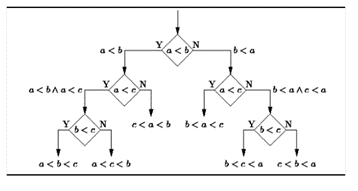
\includegraphics[scale=1.2]{img/Marco Teorico/arbol de desicion.png} 
	\label{fig:padt}
	\caption{Ejemplo de un problema aplicando Árbol de Decisiones}
\end{figure}

\par A modo de ejemplo del modelo, se puede representar de como se observa en la Figura 2.2. Las condiciones se dan como alternativas de caminos a seguir.\\

\doublespacing
\subsubsection{Usos para los Decision Tree}
\spacing{1.5}
Al ser de fácil implementación, los Decision Tree son usados en diversas áreas, siendo las instituciones financieras las más comunes, ayudando a clasificar clientes, estableciendo sus riesgos o posibilidades financieras \cite{Harrington2012}.\\
\par En el área de la salud son empleados para diagnósticos de infecciones a la sangre o predicción de ataque al corazón en pacientes de alto riesgo \cite{Harrington2012}.\\
\par En el seguimiento de movimiento, los árboles de decisión se utilizan para analizar los movimientos de un objeto en un video y predecir su ubicación en el siguiente cuadro. Esto se logra mediante la creación de un modelo de decisión que tome en cuenta factores como la velocidad, la dirección y el tamaño del objeto. \cite{Harrington2012}.\\
\par En el reconocimiento facial, los árboles de decisión se utilizan para identificar a una persona en un video o imagen. Esto se logra mediante la creación de un modelo de decisión que tome en cuenta características como la forma de la cara, el tamaño de la nariz y la distancia entre los ojos \cite{Harrington2012}.\\

\doublespacing
\subsubsection{Ventajas y Desventajas}
\spacing{1.5}
Las ventajas de esta técnica de ML es su bajo costo computacional y simple interpretación de resultados. \\
\par La mayor desventaja es que la técnica es propensa a caer en el sobreajuste, siendo a veces manipulada por quien lo implemente \cite{Harrington2012}.\\

\doublespacing
\subsection{Random Forest (Bosque Aleatorio)}
\label{sec:RF}
\spacing{1.5}
El algoritmo de Random Forest es una técnica de aprendizaje supervisado que genera múltiples árboles de decisión sobre un conjunto de datos de entrenamiento: los resultados obtenidos se combinan para obtener un modelo único más robusto en comparación con los resultados de cada árbol por separado \cite{breiman2001random}.\\
\par Cada árbol se obtiene mediante un proceso de dos etapas:

\begin{itemize}
	\item[1-.] Se genera un número considerable de árboles de decisión con el conjunto de datos. Cada árbol contiene un subconjunto aleatorio de variables $m$ (predictores) de forma que $m < M$ (donde M = total de predictores).
	\item[2-.] Cada árbol crece hasta su máxima extensión.
\end{itemize}

\par En la Figura 2.3 se muestra las etapas mencionadas anteriromente:

\begin{center}
	\begin{figure}[H]
		\centering
		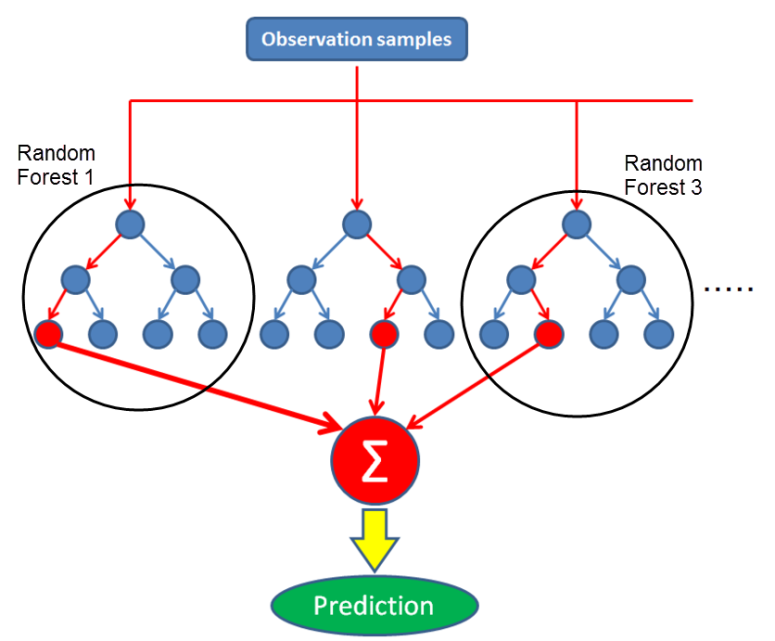
\includegraphics[scale=0.5]{img/Marco Teorico/random-forest-1.png} 
		\label{fig:Random Forest}
		\caption{Random Forest}
	\end{figure}
\end{center}


\doublespacing
\subsubsection{Ventajas y Desventajas}
\spacing{1.5}

Las principales ventajas de Random Forest son su simpleza al entrenar el modelo, desempeño muy eficiente, certera en base de datos grandes, mantiene su precisión con proporciones grandes de datos perdidos \cite{canovas2017modification}.\\
\par Algunas desventajas son la visualización gráfica donde los resultados pueden ser difíciles de interpretar, tiene poco control sobre lo que hace el modelo (en cierto sentido es como una caja negra) \cite{canovas2017modification}.\\

\doublespacing
\subsection{Naïve Bayes (Redes de Bayes)}
\label{sec:NB}
\spacing{1.5}
Naïve Bayes es un algoritmo de clasificación probabilístico que utiliza la teoría de probabilidad y estadística para realizar clasificaciones. Es llamado "Naive" porque supone que todas las características son independientes entre sí, lo que en la mayoría de los casos no es verdad. Este teorema calcula la probabilidad de una clase dada un conjunto de características. La probabilidad se calcula multiplicando la probabilidad a priori de cada clase con la probabilidad condicional de cada característica dada esa clase\cite{Vembandasamy2015}. \\
\par Este algoritmo es muy eficiente y rápido que se utiliza en una amplia gama de aplicaciones, incluyendo la detección de spam, la categorización de documentos y la clasificación de texto. Además, es uno de los algoritmos más simples y fáciles de implementar en Machine Learning \cite{Vembandasamy2015}.\\

\par La fórmula condicional se expresa en la ecuación \ref{eq:Probabilidad condicional}:\\
\begin{Large}
	\begin{equation}
		P(A|B)=\frac{P(A \cap B)}{P(B)}= \frac{(\frac{\#casos favorables A \cap B}{\#casos posibles})}{(\frac{\#casos favorables B}{\#casos posibles})}
		\label{eq:Probabilidad condicional}
	\end{equation}
\end{Large}\\
\par Desarrollando la ecuación nos queda en la ecuación \ref{eq:Probabilidad condicional resumida}\\
\begin{Large}
	\begin{equation}
		P(A|B)=\frac{P(B|A)*P(A)}{P(B)}
		\label{eq:Probabilidad condicional resumida}
	\end{equation}
\end{Large}\\
\par Donde cada evento es tomado como se demuestra en la ecuación \ref{eq:Probabilidadn del evento}\\
\begin{large}
	\begin{equation}
		P(A|B)= P(B_{1}|A) \times P(B_{2}|A) \times … \times P(B_{n}|A) \times P(A)
		\label{eq:Probabilidadn del evento}
	\end{equation}
\end{large}\\
\par $P(A|B)$ es la probabilidad posterior de la clase (objetivo) dado el predictor (atributo).
\par $P(A)$ es la probabilidad previa de clase.
\par $P(B|A)$ es la probabilidad, que es la probabilidad de la clase dada del predictor.
\par  $P(x)$ es la probabilidad previa del predictor.\\

\par Las Redes de Bayes se generan de reglas de decisión donde participan activamente las probabilidades que ocurren referente a eventos, siendo que en base a esas probabilidades y resultados obtenidos, se toman decisiones sobre cual arco de red moverse, al final del proceso, el resultado será dado por el valor del nodo final de la red \cite{Bell15}.\\
\par Considerando el gráfo mostrado en la Figura 2.4

\begin{figure}[H]
	\centering
	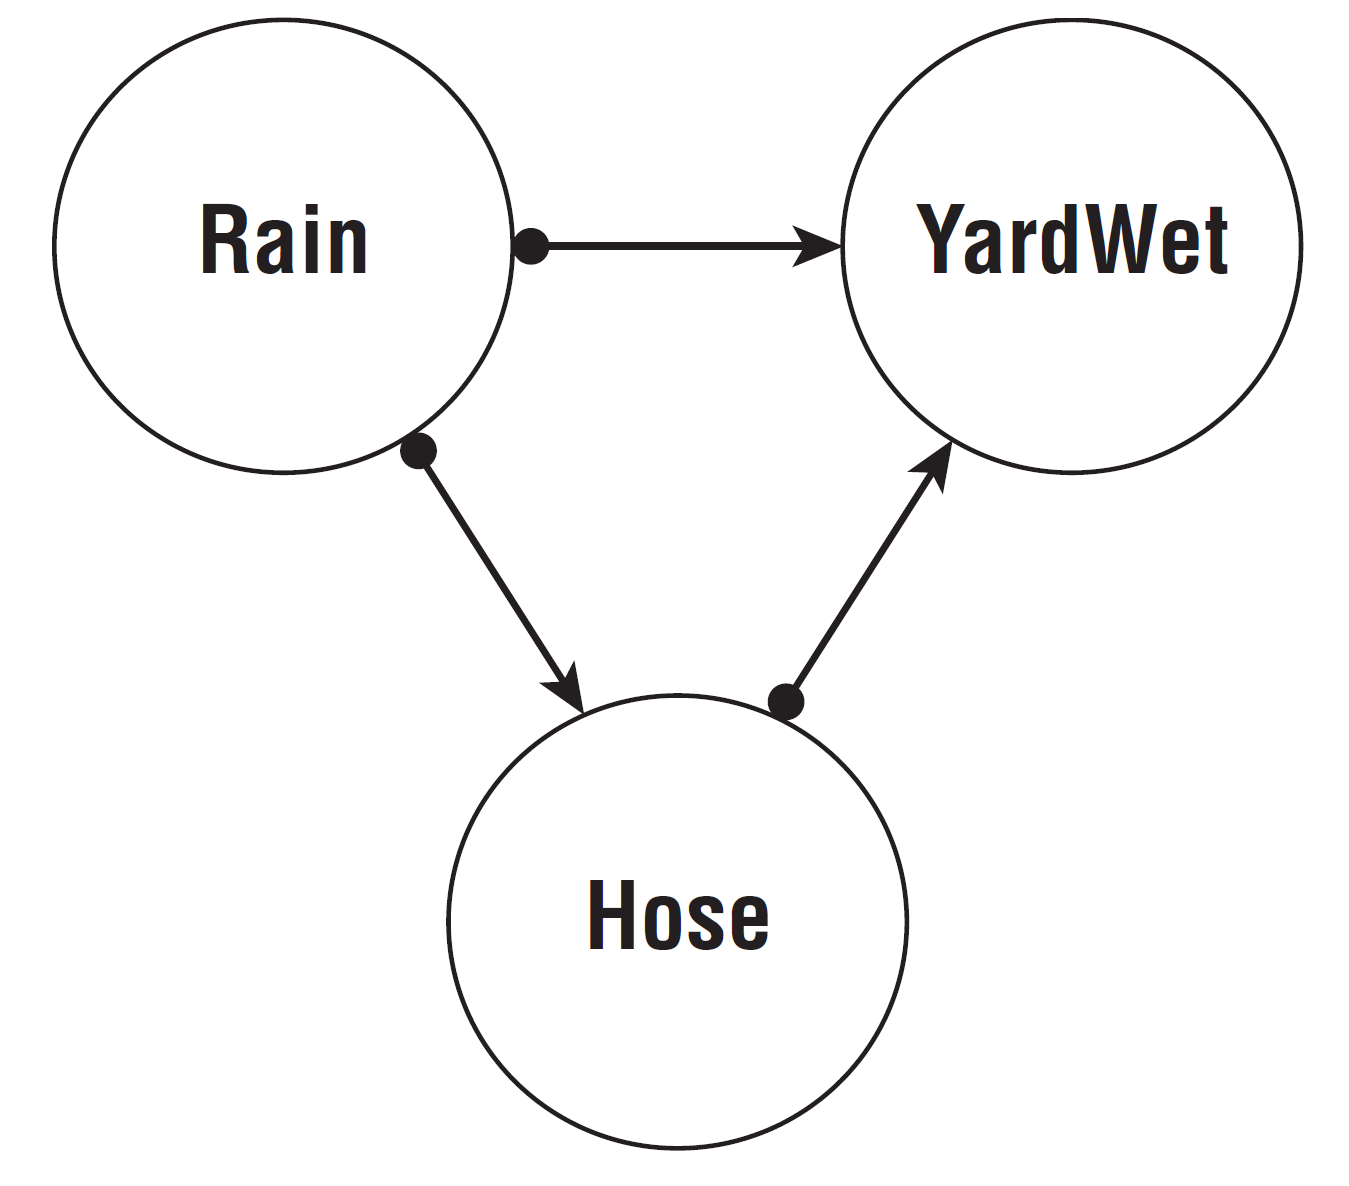
\includegraphics[scale=0.3]{img/Marco Teorico/Redes Bayes.png}  
	\label{fig:Red Bayes}
	\caption{Básica Red Bayes}
\end{figure}

\doublespacing
\subsubsection{Ventajas y Desventajas}
\spacing{1.5}
Las ventajas de esta técnica de ML son su fácilidad para implementarla, eficiencia y rápidez de tiempo de entrenamiento, buen rendimiento en textos y documentos, además no requiere mucha información para ser entrenado.\\
\par Las desventajas son la suposición a la independencia de las variables (siendo que en muchos casos las características no son independientes), vulnerable al ruido, no es óptimo para características no correlacionadas \cite{Bell15}.

\doublespacing
\subsection{Logistic Regression (Regresión Logística)}
\label{sec:LR}
\spacing{1.5}
El algoritmo Logistic Regression modela la relación entre distintas variables utilizando una medida de error que se intentará minimizar en un proceso iterativo para poder realizar predicciones acertadas, llevando a cabo una clasificación binaria con una distribución Bernoulli en vez de Gaussian y después realiza una combinación lineal de las variables en un rango de 0 a 1 \cite{ Stoltzfus2011}.\\
\par La ecuación lineal \ref{eq:Ecuación Lineal} se debe ajustar:\\
\begin{Large}
	\begin{equation}
		y(X)=W^{T}X + \epsilon = \sum_{j=1}^{D}w_{j}x_{j} + \epsilon
		\label{eq:Ecuación Lineal}
	\end{equation}
\end{Large}\\ 
\par $W^{T}X$ representa el producto escalar de entrada X.
\par $W$ e $Y$ son vectores de pesos $\in$ $\lbrace 0,1 \rbrace$.\\

\par Ahora mostrando la ecuación \ref{eq:Distribución de Bernoulli} la distribución de Bernoulli:\\
\begin{Large}
	\begin{equation}
		p(y|x,w) = Ber(y|u(x))
		\label{eq:Distribución de Bernoulli}
	\end{equation}
\end{Large}
\begin{center}
	El resultado del intervalo quedaría $0 \leq u(x) \leq 1$.\\
\end{center}
\par El resultado de la ecuación nos ayudará a predecir valores con la mejor respuesta a partir del menor error posible, teniendo un valor continuo entre 0 y 1. Si existe un valor mayor o igual a 0.5, la clase será 1, en cambio si es menor será 0. Todo esto ocurre porque el algoritmo de Logistic Regression predice un valor en vez de una clase en función de las variables utilizadas.\\

\doublespacing
\subsubsection{Ventajas y Desventajas}
\spacing{1.5}
Logistic Regression al igual que las técnicas anteriores es fácil de implementar, interpretar y muy eficiente al momento de entrenar, incluyendo que no hace suposiciones sobre distribuciones de clases en el espacio de características y es muy rápido para clasificar registros desconocidos.\\
\par Las principales desventajas de esta técnica radican en si el número de observaciones es menor que el número de características, no se debe utilizar la regresión logística; de lo contrario, puede provocar un sobreajuste y la difícil obtención de relaciones complejas.  Para trabajos más potentes y compactos existen la Artificial Neural Networks, las cuales pueden superar fácilmente este algoritmo. \cite{Harrington2012}. \\


\doublespacing
\subsection{Support Vector Machine (Máquina de Vectores de Soportes)}
\spacing{1.5}
Esta técnica no será parte de los algoritmos que se analizarán en este trabajo, sin embargo se explicará en que consiste su proceso, debido a que es una las técnicas clásicas de ML.\\ 
\par El algoritmo Support Vector Machine (SVM, por sus siglas en inglés) pertenece al ML supervisado que se utiliza para clasificación y regresión. Es un algoritmo de aprendizaje de máquina basado en el aprendizaje de modelos. El objetivo de SVM es encontrar un hiperplano que separe los datos en dos clases, de manera que los datos de una clase se encuentren en un lado del hiperplano y los datos de la otra clase se encuentren en el otro lado. El hiperplano es elegido de tal manera que maximice la margin, es decir, la distancia entre el hiperplano y los datos más cercanos. Estos datos más cercanos son conocidos como vectores de soporte. En este método, una función elige la predicción del valor esperado del caso mediante una entrada de datos \cite{Dantas2021}.\\


\doublespacing
\subsection{Artificial Neural Networks (Redes Neuronales Artificiales)}
\spacing{1.5}
Esta técnica no será parte de los algoritmos que se analizarán en este trabajo, sin embargo se explicará en que consiste su proceso, debido a que es una las técnicas clásicas de ML. \\
\par La Artificial Neural Networks (ANN, por sus siglas en inglés) son un tipo de modelo de aprendizaje automático que simula la estructura y función de las redes neuronales en el cerebro humano. Una ANN está compuesta por nodos o "neuronas" que están conectados entre sí y transmiten información a través de las conexiones. Posee posee una arquitectura de procesadores múltiples interconectados para simular la estructura humana \cite{salas2004redes}. Las ANN se utilizan para realizar tareas como la clasificación, la regresión, la traducción de idiomas, la generación de texto y la identificación de patrones en grandes conjuntos de datos.\\
\par Los métodos de aprendizaje que se emplean por lo regular son arquitecturas de redes neuronales tradicionales, donde solo se tienen dos o tres capas ocultas, imitando la operación que realiza el cerebro (Azath et al., 2020), en cambio, el DL aprenden sobre la marcha y su arquitectura puede llegar a tener 150 capas ocultas. \\

\doublespacing
\subsection{Deep Belief Network (Red de creencias profundas)}
\spacing{1.5}
Esta técnica no será parte de los algoritmos que se analizarán en este trabajo, sin embargo se explicará en que consiste su proceso, debido a que es una las técnicas clásicas de ML. \\
\par La Deep Belief Network (DBN, por sus siglas en inglés) son un tipo de ANN que se utiliza para modelar relaciones complejas entre variables. Una DBN es una combinación de varias redes neuronales artificiales y se entrena de forma no supervisada para aprender patrones y relaciones en los datos.  La DBN tiene múltiples niveles de capas y variables ocultas, ellas están conectadas entre las capas visibles y ocultas, pero no en las capas visibles – visible u oculta – oculta \cite{PuertaBarrera2015}.\\
\par Las DBN se utilizan en aplicaciones como la clasificación de imágenes, la detección de fraudes, la recomendación de productos y la identificación de tendencias en los datos. \\

\doublespacing
\subsection{Feedforward Artificial Neural Network (Red Neuronal de Retroalimentación)}
\spacing{1.5}
Esta técnica no será parte de los algoritmos que se analizarán en este trabajo, sin embargo se explicará en que consiste su proceso, debido a que es una las técnicas clásicas de ML. \\ \par Las Feedforward Artificial Neural Network (FANN) es la sucesora de ANN, trabajándose en diversos campos y aplicándose más en DL. Este algoritmo se caracteriza por tener una estructura en la que los datos fluyen en una dirección, desde las entradas hasta las salidas, sin retroalimentación o retroalimentación en ciclo. En la FANN, los datos se introducen en la red en la capa de entrada y se procesan a través de varias capas intermedias, cada una compuesta por una serie de nodos o neurones. Los nodos realizan cálculos simples en base a las entradas recibidas y generan una salida, que a su vez es procesada por la capa siguiente. La salida final de la red se produce en la capa de salida \cite{salas2004redes}.\\ 
\par La FANN utiliza en una amplia variedad de aplicaciones, incluyendo la clasificación de imágenes, la detección de fraudes, la recomendación de productos y la identificación de tendencias en los datos.\\

\doublespacing
\subsection{Recurrent Neural Networks (Redes Neuronales Recurrentes)}
\spacing{1.5}
Esta técnica no será parte de los algoritmos que se analizarán en este trabajo, sin embargo se explicará en que consiste su proceso, debido a que es una las técnicas clásicas de ML. \\
\par La Recurrent Neural Networks (RNN, por sus siglas en inglés) son un tipo de red neuronal artificial que se utiliza en el ML. A diferencia de la FANN, las RNN tienen una estructura que permite la retroalimentación, lo que les permite tomar en cuenta la secuencia temporal de los datos. Las RNN asigna parámetros únicos para representar a cada dato en una secuencia \cite{arana2021redes}, para poder tener el control y no sufrir interrupciones sobre la secuencia. Su arquitectura es multicapa que comparte pasos entre los datos espaciados secuencialmente, para poder unir la información. Su arquitectura se va incrementando con la conexión de nodos adyacentes a través de la adición de ciclos dentro de la red.\\
\par Las RNN son reconocidas por obtener información de datos secuenciales como lo son el procesamiento del lenguaje natural, videos y subtitulación de imágenes.\\


\doublespacing
\section{Deep Learning (Aprendizaje Profundo)}
\spacing{1.5}
Las técnicas de ML están limitadas en el procesamiento de los datos naturales en forma cruda y para dar solución a la problemática se creó el aprendizaje profundo. La comprensión de la IA y cómo puede llegar a igualar los comportamientos humanos, inclusive en el aprendizaje, a veces superándonos, fue un gran acontecimiento que se debe a la gran contribución de Alan Turing \cite{Carola}. El DL como subárea del ML entra en acción cuando los datos tienen demasiadas características, son enormes, se requiere de un nivel de precisión altísima y el ML no puede ofrecer completamente los resultados deseados.\\


\doublespacing
\subsection{Convolutional Neural Networks (Redes Neuronales Convolucionales)}
\spacing{1.5}
El DL ha demostrado muy buenos resultados para la resolución de problemas, en cambio, las limitaciones, sobre todo en el campo de la imagenología, ha hecho que se elabore un método diferente para que exista un análisis más preciso al momento de analizar una imagen. Este método se llama Convolutional Neural Networks (CNN), que tiene una arquitectura con mejor rendimiento para las tareas de relaciones complejas \cite{Pena-Torres}. \\
\par Desde el año 2012, las arquitecturas basadas en CNN para visión artificial han crecido muchísimo; sin embargo, no todas han sido eficientes para ocuparse en tareas de visión artificial (Figueroa Flores, 2021), siendo el Grupo de Geometría Visual (VGG) de la Universidad de Oxford \cite{Simonyan2015} una de las arquitecturas más utilizadas para las tareas de procesamiento de visión artificial. \\
\par Las CNN se forman usando tres tipos de capas, los cuales son capas convolucionales, capas de pooling y capas totalmente conectadas, como se muestra en la Figura 2.5.\\

\begin{figure}[H]
	\centering
	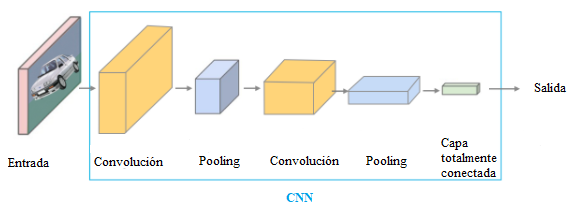
\includegraphics[scale=0.7]{img/Marco Teorico/convulcioinales.png}  
	\label{fig:CNN}
	\caption{Descripción del funcionamiento de una CNN}
\end{figure}

\par Para la CNN existen dos arquitecturas básicas, las cuales son CNN que entrega una salida para toda la imagen, como en la Figura 2.5 y la Fully Convolutional networks que posee un codificador y decodificador, entrega una compresión de la información y su salida es por pixel. En las arquitecturas CNN exiten varios ejemplos, como lo son AlexNet, entrenado con ImageNet, GoogLeNet donde posee 22 capas y sus neuronas son más complejas, entre otras \cite{NIPS2012_c399862d}.\\


\doublespacing
\subsection{Neural Networks for Scarce Data Domains  (Redes neuronales para dominios de datos escasos)}
\spacing{1.5}
Las redes neuronales pueden ser muy efectivas para abordar problemas en los que los datos son escasos \cite{Carola}. Sin embargo, cuando los datos son escasos, es esencial utilizar un enfoque diferente para entrenar las redes neuronales. Fei-Fei et al. \cite{Fei-Fei2006} demostraron que es posible aprender nuevas categorías, una o pocas muestras por clase, aprovechando las categorías aprendidas anteriormente. \\

\doublespacing
\section{Otros conceptos importantes para la investigación relacionados con la IA}
\spacing{1.5}
Existen muchos conceptos importantes que tienen relación con la IA, en esta sección tomaremos algunos que más adelante aparecerán. Estos conceptos son necesario para saber su utilización y funcionamiento.

\doublespacing
\subsection{Dataset}
\spacing{1.5}
Un Dataset se refiere a una colección de datos que generalmente tiene la misma forma que una tabla de base de datos o una hoja de cálculo \cite{Astudillo2021}. Un conjunto de datos consiste en un conjunto de ejemplos o casos. Una instancia también se denomina fila en una tabla de base de datos o, a veces, como un caso en estadística. Las funciones (columnas de la tabla) también tienen muchos nombres diferentes. Los estadísticos llaman atributos a las variables independientes o predictoras que se proporcionan como entradas. En la investigación de operaciones, también se habla de variables explicativas. La variable objetivo cuyo valor se va a predecir generalmente se denomina variable dependiente en estadística. La terminología puede ser un poco confusa; las variables independientes pueden no ser independientes entre sí (o de nada), y las variables dependientes no necesariamente dependen de todas las variables independientes. Es importante ser claro: la variable objetivo no se utiliza para predecirse a sí misma. Sin embargo, los valores anteriores de la variable objetivo pueden ser útiles para predecir valores futuros, por lo que estos valores pasados pueden incluirse como función \cite{provost2013data}.\\
\par En el Dataset la reducción de datos es importante y éste intenta tomar un gran conjunto de datos y reemplazarlo con un conjunto de datos más pequeño que contiene la mayor parte de la información importante en el conjunto más grande. Los conjuntos de datos más pequeños pueden ser más fáciles de manejar o manejar. Cuanto más pequeño sea el conjunto de datos, mejor información podrá descubrir. Por ejemplo, grandes conjuntos de datos sobre los consumidores de las preferencias de visualización de películas, estos se pueden reducir a un conjunto de datos más pequeño, que revela las preferencias de gustos del consumidor ocultas en los datos de visualización (como las preferencias de género de la audiencia). La reducción de datos a menudo se asocia con la pérdida de información \cite{provost2013data}.\\

\doublespacing
\subsection{Matriz de Confusión}
\label{sec:mc}
\spacing{1.5}
En el campo de la IA, en especial en el problema de la clasificación estadística, una matriz de confusión es una herramienta que permite la visualización del desempeño de un algoritmo que se emplea en aprendizaje supervisado .
\par La estructura de la matriz de confusión 2x2 o más (dependiendo del número de clases), donde cada fila representa una clase real y cada columna representa una clase predicha por el modelo \cite{Harrington2012}:

\begin{itemize}
	\item \textbf{Positivo (P)}: La observación es positiva (por ejemplo, el paciente \textit{tiene} COVID).
	\item \textbf{Negativo (N)}: La observación no es positiva (por ejemplo, el paciente \textit{no tiene} Covid).
	\item \textbf{Verdadero Positivo (TP)}: Resultado en el que el modelo \textit{predice correctamente la clase positiva}.
	\item \textbf{Verdadero Negativo (TN)}: Resultado donde el modelo \textit{predice correctamente la clase negativa}.
	\item \textbf{Falso Positivo (FP)}: También llamado error de tipo 1, resultado donde el modelo \textit{predice incorrectamente la clase positiva cuando en realidad es negativa}.
	\item \textbf{Falso Negativo (FN):} También llamado error de tipo 2, un resultado en el que el modelo \textit{predice incorrectamente la clase negativa cuando en realidad es positiva}.
\end{itemize}

\par La matriz de confusión se utiliza para calcular métricas de rendimiento como la precisión, la exhustividad y la medida F1.

\doublespacing
\section{Aspectos de la salud y la enfermedad}
\spacing{1.5}
La salud es una de los aspectos más importantes en la vida, muchas veces nuestra salud se ve afectada por factores externos o internos a nuestra persona. “Este concepto involucra un estado completo de bienestar físico, mental y social, y no solamente la ausencia de afecciones o enfermedades” (Wold Health Organization, 1946).  \\

\doublespacing
\subsection{Accidente Cerebro Vascular}
\spacing{1.5}
\par Un Accidente Cerebro Vascular es la detención del flujo de sangre a una parte del cerebro. En ocasiones se le llama “Ataque Cerebral”. Si el flujo sanguíneo se detiene por más de pocos segundos, el cerebro no recibirá nutrientes ni oxígeno, causando una muerte y un daño permanente en la zona afectada \cite{Garcia2019}.
\par Existen dos tipos de ACV, Isquémicos y Hemorrágicos.\\

\doublespacing
\subsection{Accidente Cerebro Vascular Isquémico}
\spacing{1.5}
\par Los ACV son los más comunes, generalmente, son causados por un coágulo sanguíneo (masas que se presentan cuando la sangre se endurece, pasando de líquida a sólida) que bloquea el vaso sanguíneo del cerebro, lo que provoca la muerte de células cerebrales. Esto puede causar daño cerebral y resultar en una variedad de síntomas y discapacidades, incluyendo debilidad en un lado del cuerpo, problemas de habla, visión doble, pérdida de la capacidad de caminar y, en casos graves, la muerte \cite{Adams1993}.\\
\par Existen dos tipos de ACV Isquémicos: transitorios y permanentes \cite{Garcia2019}. Los transitorios se producen cuando la sangre no llega al cerebro por unos instantes, en cambio, el permanente es producido cuando la sangre no llega al cerebro por un tiempo prolongado, también este llamado Infarto Cerebral. \\

\doublespacing
\subsection{Síntomas ACV Isquémico}
\spacing{1.5}
\par Los síntomas de un ACV Isquémico pueden ser:
	\begin{itemize}
		\item Entumecimiento o debilidad repentina de la cara, brazo o pierna (especialmente en un lado del cuerpo).
		\item Confusión repentina, dificultad para hablar o entender el lenguaje.
		\item Dificultad repentina para ver con uno o ambos ojos.
		\item Problemas para caminar repentino, mareos, pérdida de equilibrio o coordinación.\\
	\end{itemize}
	
\doublespacing
\subsection{Categorías de los ACV}
\spacing{1.5}
\par En los ACV para ayudar a optimizar el tratamiento específico, existen categorías que son identificadas por la escala de TOAST \cite{Adams1993}.\\
\par La primera categoría es la enfermedad Aterotrombótica aterosclerótica de gran vaso, se basa en la reducción de tejido sanguíneo medio o grande en el cerebro, con ubicación cortical o subcortical, con localización vertebrobasilar o carotídea, donde se encuentra presente una aterosclerosis u obstrucción con estenosis u oclusión de las arterias craneales. También la aterosclerosis sin estenosis con menos factores de riesgo se puede encontrar presente en esta categoría. La segunda categoría es el Cardioembolismo, es una reducción de tejido sanguíneo medio o grande, de localización cortical, en la que existe una cardiopatía embolígena \cite{Molina2018}. La tercera categoría es la enfermedad oclusiva de pequeño vaso infarto lacunar, es una reducción de tejido sanguíneo de tamaño pequeño, en el sector de una arteria perforante cerebral que puede provocar una oclusión en el transporte de nutrientes. La cuarta categoría se debe a otras causas, de tamaño o localización variable que no están en las tres categorías anteriores, y que pueden producir enfermedades metabólicas, alteraciones de la coagulación, displacia fibromuscular, etc. La quinta categoría hace énfasis a los orígenes desconocidos con estudios incompletos o completos, por más de una etiología \cite{Radu2017}.\\


\doublespacing
\subsection{Tratamiento en los ACV}
\spacing{1.5}
Las ayudas diagnósticas, proveen información sobre el grado de lesión y la identificación de la lesión  como las imágenes, escogiendo el tratamiento más adecuado para la lesión \cite{Wintermark2013}. En el tratamiento como recomendación general, el soporte de la vía aérea y la asistencia ventilatoria es fundamental, ya que los pacientes pueden presentar alteración en el estado de conciencia o disfunción bulbar que afecte la vía aérea. Además se recomienda lograr saturaciones de oxigeno mayores a 94\% aún si implica oxigeno suplementario. Agregando a lo anterior se debe monitorizar la hiperglicemia, porque si llega a perdurarpor más de 24 horas, el pronóstico se asocia a un peor desenlace \cite{Garcia2019}.\\
\par El tratamiento específico para un ACV Isquémico depende del tamaño y la ubicación del coágulo, así como de la gravedad de los síntomas. Algunos pacientes pueden requerir terapia médica, como anticoagulantes o medicamentos que disuelvan el coágulo, mientras que otros pueden necesitar cirugía o procedimientos endovasculares para extraer o disolver el coágulo. Además del tratamiento médico, los pacientes que han sufrido un ACV isquémico pueden necesitar rehabilitación para recuperar la función cerebral y física perdida. Esto puede incluir terapia física, terapia ocupacional, terapia de habla y otros tipos de rehabilitación \cite{Garcia2019}.\\


\doublespacing
\subsection{Escala de ACV del National Institute of Health (NIHSS)} 
\label{sec:NIHSS}
\spacing{1.5}
La escala de NIHSS mide el daño neurológico ocasionado en el paciente con ACV. Esta escala se ha convertido en una de las herramientas más útiles para monitozar neurológicamente en Unidades de ACV, tanto en la evaluación inicial del paciente, como para su seguimiento. El seguimiento puede arrojar mejoría o empeoramiento neurológico \cite{cien2001}. \\
\par La escala contiene 11 items (desarrollada serían 15), que permiten valorar de forma rápida: funciones corticales, pares craneales superiores, función motora, sensibilidad, coordinación y lenguaje \cite{cien2001}. La escala tiene un minimo de 0 puntos y un máximo de 42 puntos.\\
\par La clasificación de la puntación se presenta de la siguiente manera (Montaner et al, 2006) \cite{montaner2006escala}:

\begin{itemize}
	\item 0 punto: sin déficit.
	\item 1 punto: déficit mínimo.
	\item 2-5 puntos: leve.
	\item 6-15 puntos: moderado.
	\item 15-20 puntos: déficit importante.
	\item > 20 puntos: grave.\\
\end{itemize}

\par La puntuación inicial tiene buen valor pronóstico \cite{heinemann1997measurement}, considerando que un NIHSS 	$\leq$ 6 corresponde con una excelente recuperación neurológica y cada incremento en un punto empeoraría la evolución \cite{Adams1993}. Pacientes con fibrilación auricular, una NIHSS $\geq$ 16 ya se considera de muy mal pronóstico \cite{frankel2000predicting}.\\